\section{Автоморфизмы графа. Планарные графы. Поток на графе}
\subsection{Автоморфизм графа}
\begin{definition}
    \textbf{Граф} - это множество точек $V$ и множество ориентированных
     рёбер $\overrightarrow{E}$,
    на которых заданы отображения $S:\overrightarrow{E} \rightarrow V$ и $t:\overrightarrow{E} \rightarrow V$ такие,
    что $t(e)=v \Rightarrow \phi(t(e)) = \phi(v)$.
\end{definition}
\begin{explanation*}
    Вот, что такое отображения выше:
    \begin{itemize}
        \item $S:\overrightarrow{E} \rightarrow V$ - функция, возвращающая
        начало ребра
        \item$t:\overrightarrow{E} \rightarrow V$ - функция, возвращающая конец ребра
        \item Последние условие на отображения говорит нам о сохранении структуры графа
    \end{itemize}
\end{explanation*}

\begin{definition}
    \textbf{Изоморфизм графов} - это биективное отображение графа $G$ на граф $H$ с сохранением
    структуры.
\end{definition}
\begin{explanation*}
    Пусть $G, H$ - графы, тогда биективные отображения
        $$\phi : V_{G} \rightarrow V_{H}$$
        $$\psi : \overrightarrow{E}_{G} \rightarrow \overrightarrow{E}_{H}$$
задающие биекции, с сохранением структуры, задают изоморфизм.
\end{explanation*}
\textbf{Пример:} даны графы $G, H$ соответственно

\begin{tikzpicture}
    \begin{scope}[every node/.style={circle,thick,draw}]
        \node[shape=circle,draw=black] (A) at (0,1.5) {$a$};
        \node[shape=circle,draw=black] (B) at (-1.5,0) {$b$};
        \node[shape=circle,draw=black] (C) at (-1.25,-2) {$c$};
        \node[shape=circle,draw=black] (D) at (1.25,-2) {$d$};
        \node[shape=circle,draw=black] (E) at (1.5,0) {$e$};
    \end{scope}
    
    \begin{scope}[every node/.style={circle,thick,draw}]
    \path (A) edge (B);
    \path (A) edge (E);
    \path (B) edge (C);
    \path (E) edge (D);
    \path (D) edge (C);
    \end{scope}

    \begin{scope}[every node/.style={circle,thick,draw}]
        \node[shape=circle,draw=black] (A) at (6,1.5) {$\alpha$};
        \node[shape=circle,draw=black] (B) at (6-1.5,0) {$\varepsilon$};
        \node[shape=circle,draw=black] (C) at (6-1.25,-2) {$\delta$};
        \node[shape=circle,draw=black] (D) at (6+1.25,-2) {$\gamma$};
        \node[shape=circle,draw=black] (E) at (6+1.5,0) {$\beta$};
    \end{scope}
    \begin{scope}[every node/.style={circle,thick,draw}]
        \path (A) edge (D);
        \path (A) edge (C);
        \path (E) edge (B);
        \path (E) edge (C);
        \path (B) edge (D);
    \end{scope}

    \node[text width=6cm, anchor=west, right] at (7.5,0)
    {
        \begin{multline*}
            \phi : V_{G} \rightarrow V_{H}\text{ - биективное отображение, тогда:}\\
            \phi(a) = \alpha,\\
            \phi(b) = \gamma, \\
            \phi(c) = \varepsilon, \\
            \phi(d) = \beta, \\
            \phi(e) = \delta\\
        \end{multline*}
    };
\end{tikzpicture}
\\
\begin{definition}
    \textbf{Автоморфизм} - изоморфизм графа с собой.
\end{definition}

\textbf{Пример:}

\begin{tikzpicture}
    \begin{scope}
        \node[shape=circle,draw=black] (A) at (0,0) {$A$};
        \node[shape=circle,draw=black] (B) at (4,0) {$B$};
        \node[text width=6cm, anchor=north, right] at (0, -1){Это 
        очень простой граф};
        \node[text width=8cm, anchor=east, right] at (6, 0){
            Определим два отображения, задающих автоморфизм:\begin{enumerate}
                \item $\phi(a) = a$, $\phi(b) = b$\\ т.е. $\phi=Id$ ($Id$ - тождественное отображение) 
                \item $\psi(a) = b$, $\psi(b) = a$\\ $\psi$ - \textbf{автоморфизм}, но не тождественное
                отображение
            \end{enumerate}
        };
    \end{scope}
    \begin{scope}
        \path (A) edge (B);
    \end{scope}
    % \draw[red, thick][->] (1,1) arc (0:360:0.5);
    % \draw[black, ultra thick][<-] (1,1) arc (0:360:1);
    % \fill[yellow] (1,1) circle (2pt);
\end{tikzpicture}
\newpage
Теперь займёмся подсчётом \textbf{автоморфизмов}(симметрий, но не в школьном понимании) в более сложных графах:
\begin{enumerate}
    \item 
    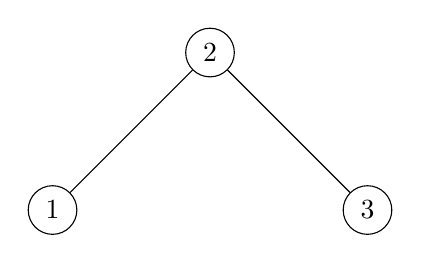
\begin{tikzpicture}
        \begin{scope}
            \node[shape=circle, draw=black] (1) at (2,0) {2};
            \node[shape=circle, draw=black] (2) at (0,-2) {1};
            \node[shape=circle, draw=black] (3) at (4,-2) {3};
            %\node[text width=12cm, anchor=east, right] at (6, 0){};
        \end{scope}
        \begin{scope}
            \path (1) edge (2);
            \path (1) edge (3);
        \end{scope}
    \end{tikzpicture}
    \begin{claim*}
        Вершина №2 может отображаться только в себя, т.к. у неё единственной в множестве вершин этого графа
        2 валентности. Вершины №1 и №3 могут отображаться как в себя, так и в друг друга, поэтому имеем два автоморфизма:
        тождественный и задающийся подстановкой 
        $\begin{pmatrix}
            1&2&3\\
            3&2&1
        \end{pmatrix}$.

        Получим, что группа автоморфизмов графа имеет мощность 2, и состоит соответственно из тождественного
        отображения и указанной выше подстановки:
        $$
        AutG = \{Id, 
        \begin{pmatrix}
            1&2&3\\
            3&2&1
        \end{pmatrix}
        \}
        $$
    \end{claim*}
    \begin{explanation*}
        Можно подумать и по-другому. Автоморфизм отображает не только вершины, но и рёбра, поэтому давайте 
        размыслим в категориях рёбер: сколькими способами можно переставить рёбра в заданном графе так, 
        чтобы не изменить его структуру, т.е. так, чтобы у каждого ребра сохранилось количество инцидентных 
        ему рёбер и его направление? Имеем, что рёбра могут быть отражены зеркально относительно вершины №2
        или же остаться на месте, т.е. имеем всего 2 варианта. Это и есть ответ.
    \end{explanation*}
    \item 
    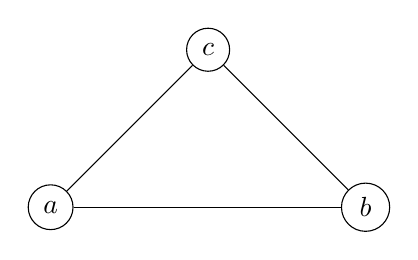
\begin{tikzpicture}
        \begin{scope}
            \node[shape=circle, draw=black] (1) at (2,0) {$c$};
            \node[shape=circle, draw=black] (2) at (0,-2) {$a$};
            \node[shape=circle, draw=black] (3) at (4,-2) {$b$};
            %\node[text width=12cm, anchor=east, right] at (6, 0){};
        \end{scope}
        \begin{scope}
            \path (1) edge (2);
            \path (1) edge (3);
            \path (2) edge (3);
        \end{scope}
    \end{tikzpicture}
    \begin{claim*}
        Каждая из вершин имеет по две валентности, следовательно, без нарушения структуры она может отобразиться в себя
        и в любую соседнюю вершину. Имеем $3!$ возможностей и $|AutG| = 6$.
    \end{claim*}
    \item 
    \begin{tikzpicture}
        \begin{scope}
            \node[shape=circle, draw=black] (1) at (2,-2) {2};
            \node[shape=circle, draw=black] (2) at (0,0) {1};
            \node[shape=circle, draw=black] (3) at (4,0) {3};
            \node[shape=circle, draw=black] (4) at (2,-4) {4};
            %\node[text width=12cm, anchor=east, right] at (6, 0){};
        \end{scope}
        \begin{scope}
            \path (1) edge (2);
            \path (1) edge (3);
            \path (1) edge (4);
        \end{scope}
    \end{tikzpicture}
    \begin{claim*}
        Вершина №2 единственная с тремя валентностями, поэтому отображаться с сохранением
        структуры она может только в себя. Остальные вершины могут без ограничений отображаться
        друг в друга, поэтому имеем ситуацию как с треугольником выше.
    \end{claim*}
    \begin{notice}
        Петля на самом деле имеет два автоморфизма:
        \begin{center}
            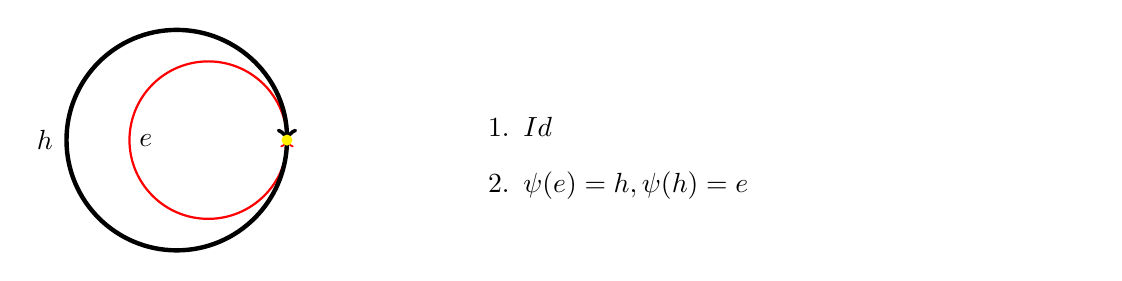
\begin{tikzpicture}
                \begin{scope}
                    \draw[red, thick][->] (1,1) arc (0:360:1);
                    \draw[black, ultra thick][<-] (1,1) arc (0:360:1.4);
                    \fill[yellow] (1,1) circle (2pt);
                \end{scope}
                \begin{scope}
                    \node[text width=2cm, anchor=west, right] at (-2.3,1){$h$};
                    \node[text width=2cm, anchor=west, right] at (-1,1){$e$};
                    \node[text width=8cm, anchor=west, right] at (3,1){
                    \begin{enumerate}
                        \item $Id$
                        \item $\psi(e) = h, \psi(h) = e$
                    \end{enumerate}
                    };
                \end{scope}
            \end{tikzpicture}
        \end{center}
    \end{notice}
    \item
    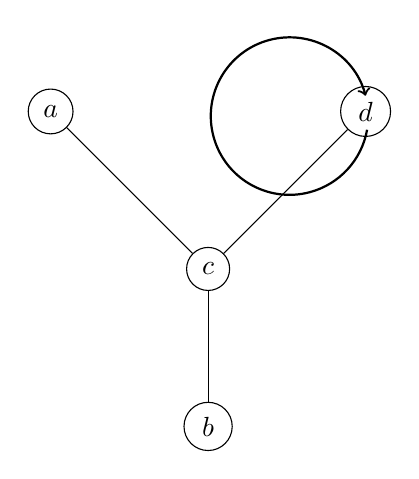
\begin{tikzpicture}
         \begin{scope}
            \draw[black, thick][<-] (4,0.2) arc (15:350:1);
        \end{scope}
        \begin{scope}
            \node[shape=circle, draw=black] (1) at (2,-2) {$c$};
            \node[shape=circle, draw=black] (2) at (0,0) {$a$};
            \node[shape=circle, draw=black] (3) at (4,0) {$d$};
            \node[shape=circle, draw=black] (4) at (2,-4) {$b$};
            %\node[text width=12cm, anchor=east, right] at (6, 0){};
        \end{scope}
        \begin{scope}
            \path (1) edge (2);
            \path (1) edge (3);
            \path (1) edge (4);
        \end{scope}
    \end{tikzpicture}
    \begin{claim*}
        Петлю можно повернуть двумя способами, вершина $c$ может отобразиться только в себя - см. предыдущий пункт - остаётся 
        перестановка вершин $a$ и $b$ - их можно расставить двумя способами:
        не перемещая или отобразив друг в друга. Итого $2*2=4$.
    \end{claim*}
    \item 
    \begin{tikzpicture}
        \begin{scope}
            \node[shape=circle, draw=black] (1) at (0,0) {1};
            \node[shape=circle, draw=black] (2) at (2,-2) {2};
            \node[shape=circle, draw=black] (3) at (6,-2) {3};
            \node[shape=circle, draw=black] (4) at (8,0) {4};
            \node[shape=circle, draw=black] (5) at (8,-4) {5};
            \node[shape=circle, draw=black] (6) at (0,-4) {6};
        \end{scope}
        \begin{scope}
            \path (1) edge (2);
            \path (2) edge (3);
            \path (3) edge (4);
            \path (3) edge (5);
            \path (6) edge (2);
        \end{scope}
    \end{tikzpicture}
    \begin{claim*}
        Вершины №1 и №6 можно расставить двумя способами. Аналогично с вершинами №4 и №5.\\
        Теперь про вершины №2 и №3: здесь важно, чтобы отображение вершины №2 было инцидентно ребрам, на которые отобразились вершины №1 и №6. Аналогичное условие накладывается на вершину №3. Поэтому для них есть только 2 возможности: либо они отображаются в себя, либо мы отражаем граф относительно центра ребра, соединяющего вершины №2 и №3. \textbf{Итого:} $2*2*2=8$ отображений.
    \end{claim*}
    \item
    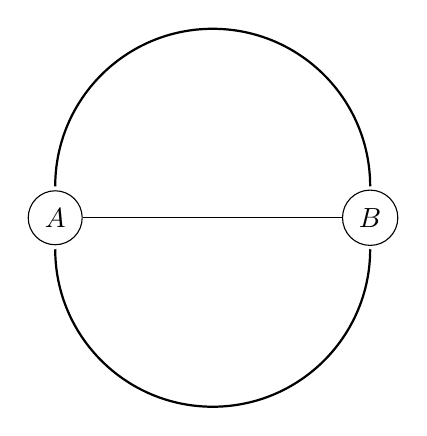
\begin{tikzpicture}
    \begin{scope}
        \node[shape=circle,draw=black] (A) at (0,0) {$A$};
        \node[shape=circle,draw=black] (B) at (4,0) {$B$};
    \end{scope}
    \begin{scope}
        \path (A) edge (B);
        \draw[black, thick] (4,0.4) arc (0:180:2);
        \draw[black, thick] (0,-0.4) arc (180:360:2);
    \end{scope}
\end{tikzpicture}
\begin{claim*}
    Все три ребра здесь идентичны, поэтому берём сразу $3!$ способа их расставить. Но их можно ещё и перевернуть, поэтому количество возможных комбинаций удваивается. \textbf{Итого:} $3!*2=12$ вариантов.
\end{claim*}
\end{enumerate}
\newpage
\subsection{Планарные графы}
\begin{definition}
    \textbf{Планарным} называется граф, который можно вложить в плоскость без самопересечений.
\end{definition}
\begin{explanation*}
    Самопересечения - это ситуации, когда на графе есть ситуации с пересечением рёбер, которые в принципе то пересекаться не должны, т.е. на этом пересечении нет вершины.
\end{explanation*}

\textbf{Пример:}

\begin{tikzpicture}
    \begin{scope}
        \node[shape=circle,draw=black] (A) at (0,0) {$a$};
        \node[shape=circle,draw=black] (B) at (3,0) {$b$};
        \node[shape=circle,draw=black] (C) at (3,-3) {$c$};
        \node[shape=circle,draw=black] (D) at (0,-3) {$d$};
        \draw[thick, ->, black] (4,-1.5) -- (9,-1.5);
    \end{scope}
    \begin{scope}
        \path (A) edge (B);
        \path (A) edge (C);
        \path (B) edge (D);
        \path (B) edge (C);
        \path (C) edge (D);
        \path (A) edge (D); 
    \end{scope}
    \begin{scope}
        \node[text width=6cm, anchor=west, right] at (-1, -5){
            Этот граф вложен в плоскость с самопересечениями.\\
            Попробуем это исправить.
        };
        \node[text width=5cm, anchor=west] at (4, -2){
            \begin{center}
                Вытащим ребро $bd$ наружу.
            \end{center}
        };
        \node[text width=4cm, anchor=west] at (14.5, -1.4){
            Теперь граф без самопересечений вкладывается в плоскость.
            Следовательно, он \textit{планарен}.
        };
    \end{scope}
    \begin{scope}
        \node[shape=circle,draw=black] (A1) at (10,0) {$a$};
        \node[shape=circle,draw=black] (B1) at (13,0) {$b$};
        \node[shape=circle,draw=black] (C1) at (13,-3) {$c$};
        \node[shape=circle,draw=black] (D1) at (10,-3) {$d$};
    \end{scope}
    \begin{scope}
        \path (A1) edge (B1);
        \path (A1) edge (C1);
        \path (B1) edge (C1);
        \path (C1) edge (D1);
        \path (A1) edge (D1); 
        \draw[thick] (13,-0.3) .. controls (15,-5).. (10,-3.3);
    \end{scope}
\end{tikzpicture}

\subsubsection{Эйлерова характеристика поверхности}
Теперь представим, что в двумерном мире на двух разных топологических объектах - торе и и сфере - живут человечки.
Им очень хочется узнать, на одинаковых ли с точки зрения топологии объектах они живут. Как это сделать, не выходя в космос?

\begin{figure}[ht]

    \centering
                    
    \includegraphics[scale=0.2]{ex1.jpg}
    \includegraphics[scale=0.17]{ex2.jpg}  
    \caption{Тор и сфера}
                    
    \label{fig:top1}
                
\end{figure}
\begin{claim*}
    Этот вопрос разрешил знаменитый Эйлер. Оказывается, человечкам на каждой планете необходимо нарисовать некоторую мозаику, разбивающую поверхность их родной топологической фигуры на грани. Такое разбиение представлено на рисунке~\ref{fig:top2}.
    \begin{figure}[ht]
        \centering
        \includegraphics[scale=0.6]{ex3.png}
        \includegraphics[scale=0.8]{ex4.png}  
        \caption{Разбиение тора и сферы на грани}
        \label{fig:top2}
    \end{figure}
    Теперь мы хотим посчитать количество граней, рёбер и вершин на этих поверхностях.\\
    На сфере получается $3+1=4$ граней ($3$ образованы замкнутой ломаной, которую мы начертили, и ещё одна - это внешняя грань, можно сравнить с <<мировым океаном>> на карте), $7$ вершин и $9$ рёбер. \textbf{Итого: }$В = 7, Р = 9, Г = 4$.
    
    Для тора имеем $В=8, Р=10, Г=2$.
    \begin{explanation*}
        Расчертив тор, как показано на рисунке~\ref{fig:top3}, мы видим, что по-прежнему на нём всего одна грань, которая присутствует по умолчанию. Почему грань осталась одна, несмотря на окружность вокруг дырки и <<ремень>> (обозначен красным цветом)? Очень просто! Посмотрим на рисунок~\ref{fig:top4}.
        
        И вот, что на Рис.~\ref{fig:top4} происходит: пусть есть некоторая точка $x$, находящаяся внутри зон, отделённых на рисунке ~\ref{fig:top3}, красной и синей чертами. И из неё мы хотим попасть в некоторую точку, находящуюся как бы в другой зоне (она отмечена просто точкой на Рис.~\ref{fig:top4}). И, как видно из того же Рис.~\ref{fig:top4}, это возможно сделать. Линией от $x$ до соответствующей точки обозначена траектория, по которой для этого надо двигаться.
        
    \begin{figure}[ht]
        \centering
        \includegraphics[scale=0.7]{ex5.jpg}
        \caption{Попытка получить на торе более одной грани по умолчанию}
        \label{fig:top3}
    \end{figure}
    \begin{figure}[ht]
        \centering
        \includegraphics[scale=0.35]{ex6.png}
        \caption{Иллюстрация, почему в Рис.~\ref{fig:top3} одна грань}
        \label{fig:top4}
    \end{figure}
    
    Именно поэтому и нужно ввести ещё одну ломаную линию, чтобы получить полноценную замкнутую грань.
    \end{explanation*}
    Теперь посчитаем Эйлерову характеристику данных объектов. Утверждается, что, если объекты топологически эквивалентны, т.е. совпадают с точностью до конечного числа гомеоморфных преобразований, то их Эйлерова характеристика совпадёт.\\
    Эйлерова характеристика вычисляется следующим образом:
    \begin{equation}\label{chEu} 
        В-Р+Г
    \end{equation}
    \textbf{Считаем:}
    $$
    \text{Сфера: } В-Р+Г=2;
    $$
    $$
    \text{Тор: } В-Р+Г=0;
    $$
    Следовательно, сфера и тор - это топологически разные объекты.
\end{claim*}
\begin{notice}
    Эйлерова характеристика тора с двумя дырками $-2$.
\end{notice}
Теперь про ещё один интересный факт, который нам пригодится дальше:
\begin{center}
    \begin{tikzpicture}
        \begin{scope}
            \draw(1,1) circle (3cm);
            \fill[black] (0,-1) circle (2pt);
            \fill[black] (3,1) circle (2pt);
            \fill[black] (-0.5,2) circle (2pt);
            \draw[black] (0,-1) -- (3,1);
            \draw[black] (3,1) -- (-0.5,2);
            \draw[black] (0,-1) -- (-0.5,2);
            
        \end{scope}
        \begin{scope}
            \fill[red] (1,4) circle (4pt);
            \draw[red] (1,4) -- (3,1);
            \draw[red] (1,4) -- (0,-1);
            \draw[red] (1,4) -- (-0.5,2);
            \draw[dashed, thick, red] (0,-1) -- (-0.5, -3);
            \draw[dashed, thick, red] (3,1) -- (4.5,-2);
            \draw[dashed, thick, red] (-0.5,2) -- (-4, -3);
            \fill[red] (-0.5, -3) circle (2pt);
            \fill[red] (4.5,-2) circle (2pt);
            \fill[red] (-4, -3) circle (2pt);
            \draw[red] (-0.5, -3) -- (4.5,-2);
            \draw[red] (4.5,-2) -- (-4, -3);
            \draw[red] (-4, -3) -- (-0.5, -3);
        \end{scope}
        \begin{scope}
            \draw[black] (-5,-5) -- (-4,0);
            \draw[black] (-4,0) -- (6,0);
            \draw[black] (5,-5) -- (6,0);
            \draw[black] (5,-5) -- (-5,-5);
        \end{scope}
        \node[text width=8cm, anchor=west] at (-4,-6){
           Проецирование фигуры со сферы на плоскость
        };
    \end{tikzpicture}
\end{center}

Как нетрудно убедиться, сфера эквивалентна плоскости, за исключением единственной точки, через которую ведётся проектирование (на рисунке выше - большая красная точка на сфере), которую можно без проблем отбросить. Также из рисунка видно, что граф без самопересечений проектируется со сферы на плоскость.

Из всего вышеизложенного делается вывод, что \textbf{планарный граф имеет ту же эйлерову характеристику, что и сфера}!

\textbf{Пример:}

\begin{tikzpicture}
    \begin{scope}
        \draw(0,0) rectangle (3,4);
        \draw[black] (3,4) -- (6,2);
        \draw[black] (3,0) -- (6,2);
    \end{scope}
    \begin{scope}
        \fill[black] (0,0) circle (2pt);
        \fill[black] (3,0) circle (2pt);
        \fill[black] (3,4) circle (2pt);
        \fill[black] (0,4) circle (2pt);
        \fill[black] (6,2) circle (2pt);
    \end{scope}
    \node[text width=8cm, anchor=east] at (14,2){
        \begin{enumerate}
            \item В данном графе посчитаем количество рёбер и вершин. Рёбра предлагается считать следующим образом: проходить по каждой грани и считать в ней все рёбра (получим удвоенное их количество).
            \item Получаем, что $2*Р = 12; Г=3$. 
        \end{enumerate}
        };
\end{tikzpicture}

Теперь проведём следующие рассуждения: самая маленькая грань такого графа имеет 3 ребра, следовательно, будет выполнено неравенство:
\begin{equation}\label{leqGr}
    3*Г \leq 2*Р
\end{equation}

Теперь совместим выражение \ref{chEu} для сферы и неравенство \ref{leqGr} и получим:
\begin{equation}\label{necPlan}
    Р \leq 3В - 6
\end{equation}

Выражение \ref{necPlan} является \textbf{необходимым условием планарности}.
\begin{notice}
    Как мы увидим далее, иногда это условие нужно переформулировать, чтобы добиться успеха.
\end{notice}
\newpage
\begin{problem}
    Докажем непланарность графа $V_5$ (полного графа на 5 вершинах).
\end{problem}
\begin{figure}[ht]
    \centering
    \includegraphics[scale=0.1]{ex7.png}

    \caption{$V_5$}
    \label{fig:V5}
\end{figure}
\begin{claim*}
    Естественно, проще всего сначала проверить выполнение необходимого условия планарности. 
    $В = 5$, $Р = \displaystyle\frac{В*4}{2} = 10$ - из каждой вершины исходит 4 ребра, но так мы посчитаем каждое ребро дважды, поэтому делим на $2$.
    
    Теперь подставляем получившиеся цифры в неравенство \ref{necPlan} и получаем:
    $$
    10 \leq 15-6
    $$
    Неравенство не выполняется, следовательно, граф $V_5$ не планарен.
\end{claim*}
\begin{notice}
Если проверить выполнение условия \ref{necPlan} на графе <<три соседа, три колодца>> - граф $V_{3,3}$ - полный двудольный граф на трёх вершинах - то окажется, что оно выполняется. Это не говорит о его планарности, поскольку мы проверим лишь необходимое условие. Но! Возможно переформулировать необходимое условие следующим образом:

\begin{enumerate}
    \item По т. Кёнига граф двудольный $\Leftrightarrow$ все циклы в графе имеют чётную длину. Доказательство необходимости этой теоремы очевидно, достаточности - из рассмотрения алгоритма поиска в ширину можно прийти к противоречию. 
    \item Следствием является то, что в двудольном графе цикл <<распускается>> как минимум в четырёхугольник, следовательно, неравенство \ref{leqGr} переформулируется в следующее:
    \begin{equation}
        4Г \leq 2Р
    \end{equation}
\end{enumerate}
\end{notice}

\begin{problem}
    Доказать непланарность графа Петерсена.
\end{problem}
\begin{notice}
Граф Петерсена в науке о графах примечателен тем, что, если есть подозрение, что некоторое условие может выполняться для всех без исключения графов, то его проверяют на нём. И, как правило, оно не выполняется. Если же оно выполняется, то это значит, что ты идёшь в верном направлении или ошибся при проверке на этом графе.
\end{notice}
\begin{claim*}
Рассмотрим граф в поисках в нём подграфа, гомеоморфного одному из непланарных: $V_{5}$ или $V_{3,3}$. Алгоритм прост: откидываем всё лишнее, главное - не откинуть детали того самого подграфа, который даст нам непланарность.
    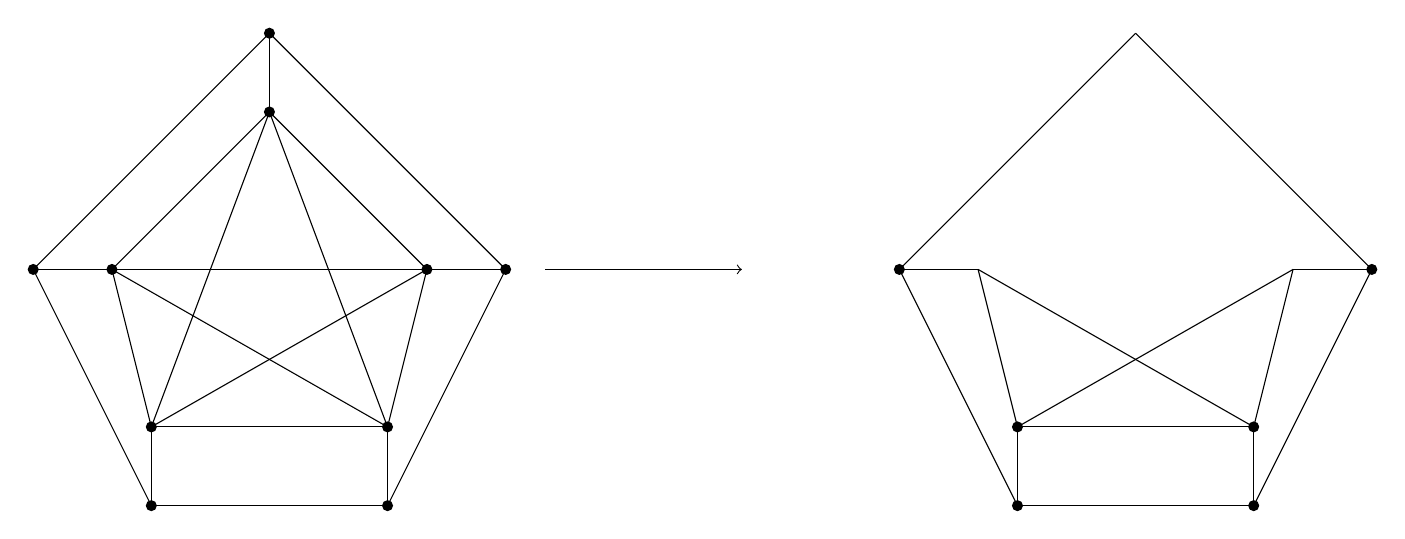
\begin{tikzpicture}
    \begin{scope}
        \draw[black] (4,0) -- (4,-1);
        \draw[black] (4,0) -- (1,-3);
        \draw[black] (4,0) -- (7,-3);
        \draw[black] (7,-3) -- (6,-3);
        \draw[black] (1,-3) -- (2,-3);
        \draw[black] (5.5,-6) -- (5.5,-5);
        \draw[black] (2.5,-6) -- (2.5,-5);
        \draw[black] (2.5,-6) -- (5.5,-6);
        \draw[black] (2.5,-6) -- (1,-3);
        \draw[black] (5.5,-6) -- (7,-3);

        \draw[black] (4,-1) -- (6,-3);
        \draw[black] (4,-1) -- (2,-3);
        \draw[black] (4,-1) -- (5.5,-5);
        \draw[black] (4,-1) -- (2.5,-5);
        \draw[black] (2,-3) -- (2.5,-5);
        \draw[black] (2,-3) -- (5.5,-5);
        \draw[black] (5.5,-5) -- (6,-3);
        \draw[black] (5.5,-5) -- (2.5,-5);
        \draw[black] (2.5,-5) -- (6,-3);
        \draw[black] (2,-3) -- (6,-3);

        \fill[black] (4,0) circle (2pt);
        \fill[black] (4,-1) circle (2pt);
        \fill[black] (1,-3) circle (2pt);
        \fill[black] (2,-3) circle (2pt);
        \fill[black] (6,-3) circle (2pt);
        \fill[black] (7,-3) circle (2pt);
        \fill[black] (2.5,-5) circle (2pt);
        \fill[black] (2.5,-6) circle (2pt);
        \fill[black] (5.5,-5) circle (2pt);
        \fill[black] (5.5,-6) circle (2pt);
    \end{scope}
    \draw[black][->] (7.5,-3) -- (10,-3);
    \begin{scope}
        \draw[black] (4+11,0) -- (1+11,-3);
        \draw[black] (4+11,0) -- (7+11,-3);
        \draw[black] (7+11,-3) -- (6+11,-3);
        \draw[black] (1+11,-3) -- (2+11,-3);
        \draw[black] (5.5+11,-6) -- (5.5+11,-5);
        \draw[black] (2.5+11,-6) -- (2.5+11,-5);
        \draw[black] (2.5+11,-6) -- (5.5+11,-6);
        \draw[black] (2.5+11,-6) -- (1+11,-3);
        \draw[black] (5.5+11,-6) -- (7+11,-3);

        \draw[black] (2+11,-3) -- (2.5+11,-5);
        \draw[black] (2+11,-3) -- (5.5+11,-5);
        \draw[black] (5.5+11,-5) -- (6+11,-3);
        \draw[black] (5.5+11,-5) -- (2.5+11,-5);
        \draw[black] (2.5+11,-5) -- (6+11,-3);

        \fill[black] (1+11,-3) circle (2pt);
        \fill[black] (7+11,-3) circle (2pt);
        \fill[black] (2.5+11,-5) circle (2pt);
        \fill[black] (2.5+11,-6) circle (2pt);
        \fill[black] (5.5+11,-5) circle (2pt);
        \fill[black] (5.5+11,-6) circle (2pt);
    \end{scope}
    \end{tikzpicture}\\
    Если немного преобразовать рёбра получившегося графа, то можно без труда увидеть, что это в точности $V_{3,3}$, следовательно, граф непланарен.
\end{claim*}
\newpage
\begin{notice}
    В завершение добавим кое-что про тор. Развёртка тора на плоскость представлена на Рис.`\ref{tikz:Tor}.
    Её можно получить, сначала <<разрезав>> тор по красной линии на Рис.~\ref{fig:top3}, 
    а затем <<разрезав>> уже получившийся <<шланг>>.
    Стрелки на рисунке указывают направление, в котором надо склеивать получившуюся развёртку, чтобы
    снова получить тор.
\end{notice}
\begin{center}
    \begin{tikzpicture}
        \draw[thick, ->, black] (0,0) -- (10,0);
        \draw[thick, <-, black] (10.1,0) -- (10.1, -5);
        \draw[thick, <-, black] (10,-5) -- (0, -5);
        \draw[thick, ->, black] (-0.1,-5) -- (-0.1, 0);
        \node[text width=8cm, anchor=north, right] at (2, -5.5){
            Рис.~\ref{tikz:Tor}: Развёртка тора на плоскости
        };
        \label{tikz:Tor}
    \end{tikzpicture}
\end{center}

\subsection{Поток на графе}
\begin{definition}
    \textbf{Поток} - это отображение $f:\overrightarrow{E} \rightarrow \mathbb{R}$
    такое, что выполняются следующие правила:

    \begin{enumerate}
        \item $f(\overrightarrow{e}) = -f(\stackrel{\leftarrow}{e})$
        \item $\forall v\in V\Rightarrow \sum\limits_{e, S(e)=v}f(e) = \sum\limits_{e, t(e)=v}f(e) =0$
    \end{enumerate}
\end{definition}
\begin{explanation*}
    Первое условие можно сформулировать так: поток ребра равен потоку, 
    взятому с этого же ребра в противоположном направлении (именно это и означает 
    противоположно направленный значок стрелки). Иными словами, мы договариваемся, что у каждого 
    ребра графа, на котором мы задаём поток, будут два направления: положительное и отрицательное. 
    Поток на них будет одинаков по модулю, но иметь противоположные знаки. Приме потока на графе 
    см. ниже.\\
    Второе условие, по сути, формулирует <<закон сохранения потока>>:
    сколько потока в вершину вошло, столько и должно выйти. В разделе физики, посвящённом электроцепям, 
    сформулировано правило Киргофа: <<сколько тока втекло, столько и вытекло>> - здесь имеем ту же ситуацию.
\end{explanation*}

\textbf{Пример:}\\
\begin{center}
    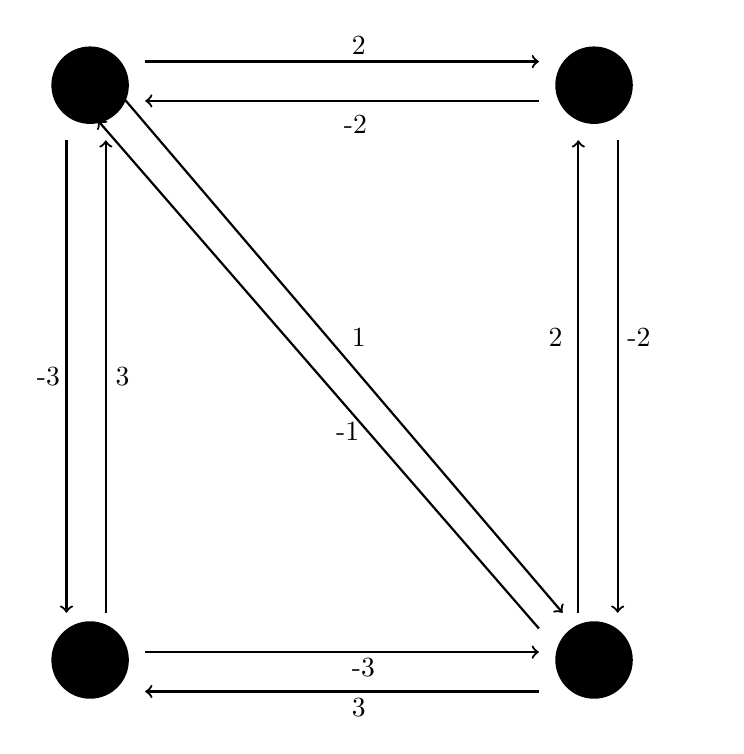
\begin{tikzpicture}
        \begin{scope}
            \draw[thick][->] (0,0) -- (5,0);
            \draw[thick][<-] (0,-0.5) -- (5,-0.5);
            \draw[thick][<-] (-1,-7) -- (-1,-1);
            \draw[thick][->] (-0.5,-7) -- (-0.5,-1);
            \draw[thick][<-] (6,-7) -- (6,-1);
            \draw[thick][->] (5.5,-7) -- (5.5,-1);
            \draw[thick][<-] (0,-8) -- (5,-8);
            \draw[thick][->] (0,-7.5) -- (5,-7.5);
            \draw[thick][->] (-0.5,-0.2) -- (5.3,-7);
            \draw[thick][<-] (-0.6,-0.75) -- (5,-7.2);
        \end{scope}
        \begin{scope}
            \fill[black] (-0.7, -0.30) circle (14pt);
            \fill[black] (5.7, -0.30) circle (14pt);
            \fill[black] (-0.7, -7.6) circle (14pt);
            \fill[black] (5.7, -7.6) circle (14pt);
        \end{scope}
        \begin{scope}
            \node[text width=1cm, anchor=west, right] at (2.5, 0.2){2};
            \node[text width=1cm, anchor=west, right] at (2.4, -0.8){-2};
            \node[text width=1cm, anchor=north, right] at (2.5, -7.7){-3};
            \node[text width=1cm, anchor=north, right] at (2.5, -8.2){3};
            \node[text width=1cm, anchor=north, right] at (5, -3.5){2};
            \node[text width=1cm, anchor=north, right] at (6, -3.5){-2};
            \node[text width=1cm, anchor=north, right] at (2.5, -3.5){1};
            \node[text width=1cm, anchor=north, right] at (2.3, -4.7){-1};
            \node[text width=1cm, anchor=west, right] at (2.5-4, -4){-3};
            \node[text width=1cm, anchor=west, right] at (2.5-3, -4){3};
        \end{scope}
    \end{tikzpicture}        
\end{center}

Потоки мы расставляли следующим образом: сначала мы указали значение потока 
для двух не смежных рёбер. И исходя и проставленных отметок, согласуясь с 
правилом Киргофа, мы уже проставили значения потоков для остальных рёбер, т.е. 
главным было правило: сколько потока в вершину втекло, столько и должно выйти.
Например: если изначально мы поставим значения потока на верхнем и на нижнем 
рёбрах $2$ и $3$ соответственно, то тогда нужно, чтобы, во-первых, в верхнее 
ребро входило потока больше, чем $2$, т.к. он ещё должен остаться на 
диагональное ребро, во-вторых, в сумме в начало нижнего ребра должен прийти 
поток $3$, но из правого бокового ребра может теперь прийти лишь $2$, следовательно,
из диагонального ребра должна прийти единица. Аналогичными рассуждениями 
получаем, что на левом боковом ребре из нижней вершины должен выходить 
поток $3$.\\
В этих рассуждениях мы не вспоминали про отрицательные потоки, хотя они должны 
быть из определения (см. первое условие, наложенное на отображение потока).  
И вот почему: они мгновенно получаются из первого условия, наложенного на отображение потока (см. 
определение), просто дорисовыванием к рёбрам графа противонаправленных рёбер 
с противополжными значениями потока.


\begin{notice}
    Далее мы не будем рисовать на потоках рёбра с отрицательным значением потока, 
    т.к. они легко получаются, при необходимости, из определения.
\end{notice}

